%\documentclass[11pt,a4paper]{article}
%\usepackage{fullpage}
%\usepackage{beamerarticle}
%\documentclass[handout,xcolor=pdftex,dvipsnames,table]{beamer}
\documentclass[hyperref={unicode=true}]{beamer}

%\usepackage{pgfpages} 
%\pgfpagesuselayout{resize}[a4paper,border shrink=5mm,landscape] 

\usepackage[utf8]{inputenc}
\usepackage[russian]{babel}
\usepackage{../clrscode3e} 
%\usepackage[all]{xy}
\usepackage{colortbl}
%\usepackage{xcolor}
\usepackage{pstricks, pst-tree, pst-node}
\usepackage{epsfig}
\usepackage{multicol}
%\usepackage{listings}

\definecolor{orange}{cmyk}{0,0.52,1,0}

%\usepackage{beamerthemesplit}

\AtBeginSubsection[]
{
  \begin{frame}<beamer>{Раздел}
    \tableofcontents[currentsection,currentsubsection]
  \end{frame}
}

%
% Добавить примеры про Бойера-Мура с l'
%
% zydxabcxabc
% abcxabcx
%     ^^^^
%



\newtheorem{rtheorem}{Теорема} 
\newtheorem{rconsequence}{Следствие} 
%default}
%themesplit}

\title{Классические алгоритмы\\ поиска образца в строке}
\subtitle{Дискретный анализ 2012/13}
\author{Андрей Калинин, Татьяна Романова}
\date{12 ноября 2012 г. }
\usetheme{default}
%\usefonttheme{serif}
\usefonttheme[onlymath]{serif}
%\usefonttheme{professionalfonts}
%\usetheme{default} 


\begin{document}

\frame{\titlepage}

%\section[Содержание]{}
\frame{\tableofcontents}

%\section{Литература}
\frame
{
  \frametitle{Литература}

  \begin{itemize}
  \item Дэн Гасфилд, <<Строки деревья и последовательности в алгоритмах:
    Информатика и вычислительная биология>>, 2003. Глава 3, <<Более глубокий взгляд>>, стр. 46--94.  
  \item Билл Смит, <<Методы и алгоритмы вычислений на строках>>,
    2006. 
  \end{itemize}
}

\section{Алгоритм Кнута-Морриса-Пратта}


\subsection{Классический вариант алгоритма}

\frame{
  \frametitle{Отличия}
  \begin{itemize}
  \item Не использует $Z$-блоки для расчёта значений $sp_i$. 
  \item Строит последовательно значения $sp_k$ по рассчитанным
    значениям от 1 до $k-1$.
  \item Легко обобщается на случай большого количества образцов
    (алгоритм Ахо-Корасик) 
  \end{itemize}
}

\frame{
  \frametitle{Обозначения}
  \begin{itemize}
  \item $\alpha$ --- префикс длиной $sp_k$, $\alpha'$ --- суффикс. 
  \item $x$ --- $k+1$-й символ.
  \item $\beta = \overline{\beta} x$ --- префикс длины $sp_{k+1}$,
    нахождение $\overline{\beta}$ эквивалентно вычислению $sp_{k+1}$.
  \end{itemize}
~\\
~\\
\includegraphics[scale=1.0]{ac.4.eps}
}

\frame{
  \frametitle{Связь $sp_{k+1}$ и $sp_k$}
  \begin{rtheorem}
    $\forall k:~sp_{k+1} \leq sp_k+1$; $sp_{k+1} = sp_k+1
    \Longleftrightarrow P(sp_k+1) = P(k+1)$
  \end{rtheorem}
  \begin{proof}
    Если $sp_{k+1}>sp_k+1$, то $|\beta|>|\alpha|$, причём $\beta$
    является одновременно префиксом $P$ и суффиксом $P[1..k]$, что
    противоречит выбору $sp_k$.
  \end{proof}
}

\frame{
  \frametitle{Общий случай}
  Если $P(k+1)\neq P(sp_k+1)$, то $sp_{k+1}\leq sp_k$ и
  $\overline{\beta}$ --- собственный префикс и суффикс $\alpha$. \\
~\\
~\\
~\\
\includegraphics[scale=1.0]{ac.3.eps}
}

\begin{frame}[fragile]
  \frametitle{Расчёт $sp_{k+1}$}
\begin{columns}
\begin{column}{.5\textwidth}
  \begin{codebox}
    \onslide<5->{
      \li $sp_1 \gets 0$
      \li \For $k \gets 1$ \To $n-1$ 
    }
    \li \Do $x \gets P(k+1)$
    \li $v \gets sp_k$
    \li \While $P(v+1)\neq x$ \func{and} $v \neq 0$
    \li \Do $v \gets sp_v$ \End
    \li \If $P(v+1) \isequal x$
    \li \Then $sp_{k+1} \gets v+1$
    \li \Else $sp_{k+1} \gets 0$ \End
    \End
  \end{codebox}
\end{column}
\begin{column}{.5\textwidth}
\begin{semiverbatim}
\onslide<2->{a\rnode{rb1}{b}\alert<4>{x}a\rnode{rb2}{b}\alert<3>{q}abxa\rnode{rb3}{b}\alert<2>{r}abxabqabxa\rnode{rb4}{b}\alert<2->{x}}
\onslide<2->{\nccurve[angleA=125,angleB=45]{->}{rb4}{rb3}}
\onslide<3->{\nccurve[angleA=125,angleB=45]{->}{rb3}{rb2}}
\onslide<4->{\nccurve[angleA=125,angleB=45]{->}{rb2}{rb1}}
\end{semiverbatim}
\end{column}
\end{columns}
\end{frame}

\frame{
  \frametitle{Линейность}
  \begin{rtheorem}
    Алгоритм находит все значения $sp_i(P)$ за время $O(n)$, где $n$
    --- длина $P$.
  \end{rtheorem}
  \begin{proof}
    Время работы пропорционально числу присваиваний $v$:
    \begin{itemize}
    \item Один раз на каждом шаге, $v \gets sp_k$. 
    \item Несколько раз уменьшается внутри \While.
    \item Число увеличений ограничено $n-1$, следовательно и число
      уменьшений ограниено $n-1$
    \item Тогда ощее число присваиваний $v$ ограничено сверху $2(n-1)=O(n)$
    \end{itemize}
  \end{proof}
}

\frame{
  \frametitle{Вычисление $sp'_i$}

  \begin{codebox}
    \li $sp'_1 \gets 0$
    \li \For $i \gets 2$ \To $n$ 
    \li \Do $v \gets sp_i$
    \li \If $P(v+1) \neq P(i+1)$
    \li \Then $sp'_i \gets v$ 
    \li \Else $sp'_i \gets sp'_v$
  \end{codebox}
}

\section{Алгоритм Ахо-Корасик}

\subsection{Задача множественного поиска}
\frame{
  \frametitle{Формулировка}
  \begin{itemize}
  \item Задано множество образцов, $\mathbb{P}=\{P_1, P_2, \ldots,
    P_z\}$. 
  \item Необходимо найти все вхождения в $T$ любых образцов из~$\mathbb{P}$.
  \item Теперь $n = \sum_{k=1}^z|P_k|$
  \item Предыдущие алгоритмы могут решить за $O(n+zm)$.
  \item Возможно решение за $O(n+m+k)$, где $k$ --- количество
    вхождений в $T$ образцов из $\mathbb{P}$
  \end{itemize}
}

\frame{
\frametitle{Дерево ключей $\mathbb{K}$}
\begin{columns}
  \begin{column}{.5\textwidth}
\pstree[treemode=R,levelsep=20pt,labelsep=2pt]{\Tdot}
{
  \pstree{\Tdot}{\taput{$p$}
    \pstree{\Tdot}{\taput{$o$}
      \pstree{\Tdot}{\taput{$t$}
        \pstree{\Tdot}{\taput{$a$}
          \pstree{\Tdot}{\taput{$t$}
            \pstree{\Tdot~{1}}{\taput{$o$}}
          }
        }
        \pstree{\Tdot}{\tbput{$t$}
          \pstree{\Tdot}{\tbput{$e$}
            \pstree{\Tdot}{\tbput{$r$}
              \pstree{\Tdot~{3}}{\tbput{$y$}
              }
            }
          }
        }
      }
      \pstree{\Tdot}{\tbput{$e$}
        \pstree{\Tdot}{\tbput{$t$}
          \pstree{\Tdot}{\tbput{$r$}
            \pstree{\Tdot~{2}}{\tbput{$y$}}
          }
        }
      }
    }
  }
  \pstree{\Tdot}{\tbput{$s$}
    \pstree{\Tdot}{\tbput{$c$}
      \pstree{\Tdot}{\taput{$h$}
        \pstree{\Tdot}{\taput{$o$}
          \pstree{\Tdot}{\taput{$o$}
            \pstree{\Tdot~{5}}{\taput{$l$}
            }
          }
        }
      }
      \pstree{\Tdot}{\tbput{$i$}
        \pstree{\Tdot}{\tbput{$e$}
          \pstree{\Tdot}{\tbput{$n$}
            \pstree{\Tdot}{\tbput{$c$}
              \pstree{\Tdot~{4}}{\tbput{$e$}
              }
            }
          }
        }
      }
    }
  }
}
\end{column}
\begin{column}{.5\textwidth}
  Дерево ключей $\mathbb{K}$ для множества образцов $\mathbb{P}=\{ potato,$ $poetry,$ $pottery,$
  $science,$ $school\}$. Дерево ключей строится за время $O(n)$.
\end{column}
\end{columns}
}

%\frame{
%  \frametitle{Включение образца}
%  \begin{columns}
%    \begin{column}{.5\textwidth}
%      \pstree[levelsep=20pt,labelsep=2pt]{\Tdot}{
%        \pstree{\Tdot}{\tlput{$p$}
%          \pstree{\TCircle{2}}{\tlput{$a$}
%            \pstree{\TCircle{1}}{\tlput{$t$}}
%          }
%        }
%      }
%    \end{column}
%    \begin{column}{.5\textwidth}
%      \pstree[levelsep=20pt,labelsep=2pt]{\Tdot}{
%        \pstree{\Tdot}{\tlput{$p$}
%          \pstree{\Tdot}{\tlput{$a$}{
%              \pstree{\TCircle{1}}{\tlput{$t$}}
%              \pstree{\Tdot}{\trput{$r$}
%                \pstree{\Tdot}{\trput{$t$}
%                  \pstree{\TCircle{2}}{\trput{$y$}
%                  }
%                }
%              }
%          }
%          }
%        }
%      }
%    \end{column}
%  \end{columns}
%}

\frame{
  \frametitle{Очевидный способ}
  \begin{itemize}
  \item Последовательно прикладывать корень дерева $\mathbb{K}$ к
    каждой позиции в тексте и пытаться пройти путь в дереве согласно
    символам текста. 
  \item Время работы $O(nm)$.
  \item Можно ли сдвигать дерево более чем на одну позицию?
  \item Для простоты: ни один образец в $\mathbb{P}$ не является
    собственной подстрокой другого образца.  
  \end{itemize}
}

\subsection{Связи неудач}

\frame{
  \frametitle{$lp(v)$}
  \begin{itemize}
    \item $\mathbb{L}(v)$ --- конкатенация символов на пути от корня
      $\mathbb{K}$ до вершины $v$ в порядке их появления. 
    \item Для любой вершины $v \in \mathbb{K}$ определим $lp(v)$ как
      длину наибольшего собственного суффикса строки $\mathbb{L}(v)$,
      которая является префиксом некоторого образца из $\mathbb{P}$.
  \end{itemize}
}

\frame{
  \frametitle{Связи неудач}
  \pstree[treemode=R,levelsep=40pt,labelsep=2pt,treefit=loose]{\Tdot}{
    \pstree{\Tdot[name=l1o]}{\taput{$o$}
      \pstree{\Tdot[name=l1ot]}{\taput{$t$}
        \pstree{\Tdot[name=l1oth]}{\taput{$h$}
          \pstree{\Tdot[name=l1othe]}{\taput{$e$}
            \pstree{\Tdot[name=l1other]~{4}}{\taput{$r$}}
          }
        }
      }
    }
    \pstree{\Tdot[name=l1t]}{\taput{$t$}
      \pstree{\Tdot[name=l1th]}{\taput{$h$}
        \pstree{\Tdot[name=l1the]}{\taput{$e$}
          \pstree{\Tdot[name=l1thea]}{\taput{$a$}
            \pstree{\Tdot[name=l1theat]}{\taput{$t$}
              \pstree{\Tdot[name=l1theate]}{\taput{$e$}
                \pstree{\Tdot[name=l1theater]~{3}}{\taput{$r$}
                }
              }
            }
          }
        }
      }
      \pstree{\Tdot[name=l1ta]}{\taput{$a$}
        \pstree{\Tdot[name=l1tat]}{\taput{$t$}
          \pstree{\Tdot[name=l1tatt]}{\taput{$t$}
            \pstree{\Tdot[name=l1tatto]}{\taput{$o$}
              \pstree{\Tdot[name=l1tattoo]~{2}}{\taput{$o$}
              }
            }
          }
        }
      }
    }
    \pstree{\Tdot}{\tbput{$p$}
      \pstree{\Tdot[name=l1po]}{\tbput{$o$}
        \pstree{\Tdot[name=l1pot]}{\tbput{$t$}
          \pstree{\Tdot[name=l1pota]}{\tbput{$a$}
            \pstree{\Tdot[name=l1potat]}{\tbput{$t$}
              \pstree{\Tdot[name=l1potato]~{1}}{\tbput{$o$}
              }
            }
          }
        }
      }
    }
  }
  \onslide<1->{\nccurve[linecolor=blue,linewidth=.25pt,angleA=-120,angleB=190,ncurvB=2,ncurvA=2,linestyle=dashed]{->}{l1po}{l1o}}
  \onslide<2->{\nccurve[linecolor=blue,linewidth=.25pt,angleA=-140,angleB=160,ncurvB=3,ncurvA=4,linestyle=dashed]{->}{l1pot}{l1ot}}
  \onslide<3->{\nccurve[linecolor=blue,linewidth=.25pt,angleA=-140,angleB=185,ncurvB=1.3,ncurvA=2.5,linestyle=dashed]{->}{l1potato}{l1o}}
  \onslide<4->{\ncline[linecolor=blue,linewidth=.25pt,linestyle=dashed]{->}{l1pota}{l1ta}}
  \onslide<5->{\ncline[linecolor=blue,linewidth=.25pt,linestyle=dashed]{->}{l1potat}{l1tat}}
  \onslide<6->{\nccurve[linecolor=blue,linewidth=.25pt,linestyle=dashed,angleA=-90,angleB=-90,ncurvA=.5]{->}{l1tat}{l1t}}
  \onslide<7->{\nccurve[linecolor=blue,linewidth=.25pt,linestyle=dashed,angleA=-90,angleB=-90]{->}{l1tatt}{l1t}}
  \onslide<8->{\ncline[linecolor=blue,linewidth=.25pt,linestyle=dashed]{->}{l1ot}{l1t}}
  \onslide<9->{\ncline[linecolor=blue,linewidth=.25pt,linestyle=dashed]{->}{l1oth}{l1th}}
  \onslide<10->{\ncline[linecolor=blue,linewidth=.25pt,linestyle=dashed]{->}{l1othe}{l1the}}
  \onslide<11->{\nccurve[linecolor=blue,linewidth=.25pt,linestyle=dashed,angleA=-90,angleB=0,ncurvA=.25]{->}{l1theat}{l1t}}
  \onslide<12->{\nccurve[linecolor=blue,linewidth=.25pt,linestyle=dashed,angleA=7,angleB=90,ncurvA=4]{->}{l1tatto}{l1o}}
  \onslide<13->{\nccurve[linecolor=blue,linewidth=.25pt,linestyle=dashed,angleA=10,angleB=90,ncurvA=2.7]{->}{l1tattoo}{l1o}}
}

\frame{
  \frametitle{Связь неудачи}
  \begin{itemize}
  \item Допустим, $\alpha$ --- суффикс строки $\mathbb{L}(v)$ длины
    $lp(v)$. Тогда существует единственная вершина в дереве ключей,
    помеченная строкой $\alpha$. (очевидно)
  \item Для вершины $v \in \mathbb{K}$ пусть $n_v$ --- единственная
    вершина в $\mathbb{K}$, помеченная суффиксом $\mathbb{L}(v)$ длины
    $lp(v)$. Если $lp(v)=0$, то $n_v$ --- корень $\mathbb{K}$.
  \item Упорядоченная пара $\langle v, n_v \rangle$ --- связь неудачи. 
  \end{itemize}
}

\frame{
  \frametitle{Использование связей неудач при поиске}
  \begin{codebox}
    \li $l \gets 1$, $c \gets 1$, $w \gets root[\mathbb{K}]$
    \li \Repeat
    \li \While есть дуга $\langle w, w' \rangle$, помеченная символом
    $T(c)$
    \li \Do \If $w'$ занумерована образцом $i$ 
    \li \Then $P_i$ встретилась в $T$ в позиции $l$ \End 
    \li $w \gets w'$, $c \gets c+1$\End
    \li \If $w \isequal root[\mathbb{K}]$
    \li \Then $c \gets c + 1$
    \li \Else $w \gets n_w$, $l \gets c-lp(w)$ \End
    \li \Until $c > m$
  \end{codebox}
}

\newcommand{\curw}[2]{\alt<#1>{\Tc*[linecolor=red,name=#2]{3pt}}{\Tdot[name=#2]}}
\begin{frame}[fragile]
  \frametitle{Пример использования связей неудач}
  
  \begin{columns}
    \begin{column}{.7\textwidth}
      \begin{center}
  \pstree[treemode=R,levelsep=20pt,labelsep=2pt,treefit=loose]{\curw{1,2,11}{l3}}{
    \pstree{\Tdot[name=l3o]}{\taput{$o$}
      \pstree{\Tdot[name=l3ot]}{\taput{$t$}
        \pstree{\Tdot[name=l3oth]}{\taput{$h$}
          \pstree{\Tdot[name=l3othe]}{\taput{$e$}
            \pstree{\Tdot[name=l3other]~{4}}{\taput{$r$}}
          }
        }
      }
    }
    \pstree{\Tdot[name=l3t]}{\taput{$t$}
      \pstree{\Tdot[name=l3th]}{\taput{$h$}
        \pstree{\Tdot[name=l3the]}{\taput{$e$}
          \pstree{\Tdot[name=l3thea]}{\taput{$a$}
            \pstree{\Tdot[name=l3theat]}{\taput{$t$}
              \pstree{\Tdot[name=l3theate]}{\taput{$e$}
                \pstree{\Tdot[name=l3theater]~{3}}{\taput{$r$}
                }
              }
            }
          }
        }
      }
      \pstree{\Tdot[name=l3ta]}{\taput{$a$}
        \pstree{\Tdot[name=l3tat]}{\taput{$t$}
          \pstree{\curw{8}{l3tatt}}{\taput{\alert<8>{$t$}}
            \pstree{\curw{9}{l3tatto}}{\taput{\alert<9>{$o$}}
              \pstree{\curw{10}{l3tattoo}~{2}}{\taput{\alert<10>{$o$}}
              }
            }
          }
        }
      }
    }
    \pstree{\curw{3}{l3p}}{\tbput{\alert<3>{$p$}}
      \pstree{\curw{4}{l3po}}{\tbput{\alert<4>{$o$}}
        \pstree{\curw{5}{l3pot}}{\tbput{\alert<5>{$t$}}
          \pstree{\curw{6}{l3pota}}{\tbput{\alert<6>{$a$}}
            \pstree{\curw{7}{l3potat}}{\tbput{\alert<7>{$t$}}
              \pstree{\Tdot[name=l3potato]~{1}}{\tbput{$o$}
              }
            }
          }
        }
      }
    }
  }
%  \nccurve[linecolor=blue,linewidth=.25pt,angleA=-120,angleB=190,ncurvB=2,ncurvA=2,linestyle=dashed]{->}{l3po}{l3o}
%  \nccurve[linecolor=blue,linewidth=.25pt,angleA=-140,angleB=160,ncurvB=2,ncurvA=3,linestyle=dashed]{->}{l3pot}{l3ot}
%  \nccurve[linecolor=blue,linewidth=.25pt,angleA=-140,angleB=185,ncurvB=1.3,ncurvA=2.5,linestyle=dashed]{->}{l3potato}{l3o}
%  \ncline[linecolor=blue,linewidth=.25pt,linestyle=dashed]{->}{l3pota}{l3ta}
  \alt<8>{\ncline[linecolor=red,linewidth=1pt]{->}{l3potat}{l3tat}}{\ncline[linecolor=blue,linewidth=.25pt,linestyle=dashed]{->}{l3potat}{l3tat}}
%  \nccurve[linecolor=blue,linewidth=.25pt,linestyle=dashed,angleA=-90,angleB=-90,ncurvA=.5]{->}{l3tat}{l3t}
%  \nccurve[linecolor=blue,linewidth=.25pt,linestyle=dashed,angleA=-90,angleB=-90]{->}{l3tatt}{l3t}
%  \ncline[linecolor=blue,linewidth=.25pt,linestyle=dashed]{->}{l3ot}{l3t}
%  \ncline[linecolor=blue,linewidth=.25pt,linestyle=dashed]{->}{l3oth}{l3th}
%  \ncline[linecolor=blue,linewidth=.25pt,linestyle=dashed]{->}{l3othe}{l3the}
%  \nccurve[linecolor=blue,linewidth=.25pt,linestyle=dashed,angleA=-90,angleB=0,ncurvA=.25]{->}{l3theat}{l3t}
%  \nccurve[linecolor=blue,linewidth=.25pt,linestyle=dashed,angleA=7,angleB=90,ncurvA=4]{->}{l3tatto}{l3o}
%  \nccurve[linecolor=blue,linewidth=.25pt,linestyle=dashed,angleA=10,angleB=90,ncurvA=2.7]{->}{l3tattoo}{l3o}
  \end{center}
\end{column}
\begin{column}{.3\textwidth}
\begin{semiverbatim}
  \alert<1>{x}\alert<2>{x}\alert<3>{p}\alert<4>{o}\alert<5>{t}\alert<6>{a}\alert<7>{t}\alert<8>{t}\alert<9>{o}\alert<10>{o}\alert<11>{x}x
\end{semiverbatim}
\end{column}
\end{columns}
\end{frame}

\frame{
  \frametitle{Корректность и линейность алгоритма}
  \begin{itemize}
  \item Доказательство аналогично приведённым соображениям для
    алгоритма Кнута-Морриса-Пратта. 
  \item Время поиска (с предположением об образцах, не являющимеся
    собственными подстроками) получается порядка $O(m)$.
  \end{itemize}
}

\frame{
  \frametitle{Построение связей неудач}
  \begin{itemize}
  \item Нужно найти для всех вершин $v$ соответствующие им $n_v$.
  \item Предположим, что $n_v$ вычислено для всех вершин, отстоящих на
    $k$ дуг от корня. 
  \item Вычисляем $n_v$ для одной из вершин $v$, остоящих на $k+1$ дуг
    от корня. 
  \end{itemize}
}

\frame{
  \frametitle{Функция неудач узла $v$}
  \begin{columns}
    \begin{column}{.5\textwidth}
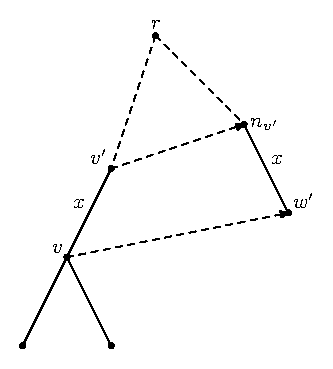
\includegraphics[scale=1.0]{ac.2.eps}
\end{column}
\begin{column}{.5\textwidth}
  \begin{itemize}
    \item $v'$ --- отец $v$ в $\mathbb{K}$.
    \item $n_{v'}$ --- известно, т.к. $v'$ отстоит на $k$ дуг от
      корня. 
    \item $x$ --- символ на дуге $\langle v', v \rangle$.
    \item Нужно проверить, есть ли дуга $\langle n_v', w' \rangle$,
      помеченая символом $x$.
      \item Если есть, то $n_v \gets w'$.
      \item В противном случае $\mathbb{L}(n_v)$~--- собственный
      суффикс $\mathbb{L}(n_{v'})$, за которым следует~$x$.
  \end{itemize}
\end{column}
\end{columns}
}

\frame{
  \frametitle{Построение связей неудач}
  \begin{codebox}
    \li $v'$ --- отец $v$ в $\mathbb{K}$, $x$ --- символ на дуге
    $\langle v', v \rangle$.
    \li $w \gets n_{v'}$
    \li \While нет дуги, выходящей из $w$, помеченной $x$ и $w \neq r$
    \li \Do $w \gets n_w$ \End
    \li \If есть дуга, выходящая из $w$ и помеченная $x$
    \li \Then $n_v \gets w'$
    \li \Else $n_v \gets r$ \End
  \end{codebox}
}

\frame{
  \frametitle{Линейность построения связей неудач}
  \begin{rtheorem}
    Полное время, затрачиваемое алгоритмом построения связей неудач в
    применении его ко всем вершинам из $\mathbb{K}$ равно $O(n)$.
  \end{rtheorem}
  \begin{proof}
    \begin{itemize}
    \item Изменение $lp(v)$ при выполнении алгоритма по пути одного
      образца $P$ длиной $t$. 
    \item $lp(v) \leq lp(v')+1$, следовательно $lp(v)$ увеличивается
      не более чем на $t$.
    \item При уменьшении $lp(v)\geq 0$ и внутренний цикл не может
      выполняться более $t$ раз. 
    \item Следовательно, связи неудач по пути $P$ находятся за время
      $O(t)$, а все связи --- за $O(n)$.
    \end{itemize}
  \end{proof}
}

\subsection{Полный алгоритм поиска}

\frame{
  \frametitle{Снятие предположения о подстроках}
  Пример: $\mathbb{P} = \{acatt, ca\}$, $T=acatg$: образец $ca$ не
  будет найден. 
  \pause
  \begin{rtheorem}
    \begin{enumerate}
    \item Пусть в дереве ключей $\mathbb{K}$ существует путь из связей
    неудач от вершины $v$ к вершине, занумерованной образцом
    $i$. Тогда в $T$ должен обнаружиться образец $P_i$, который
    оканчивается в позиции $c$ (текущий символ), как только во время
    фазы поиска алгоритма Ахо-Корасик будет достигнута вершина $v$. 
    \pause
    \item И
    наоборот: если в ходе работы достигнута вершина $v$, то образец
    $P_i$ появляется в $T$, заканчиваясь в позиции $c$, только если $v$
    имеет номер $i$ или существует путь из связей неудач из $v$ в
    вершину с номером $i$.
    \end{enumerate}
  \end{rtheorem}
}

\frame{
  \frametitle{Путь от $potat$ до $at$ через $tat$}
  \pstree[treemode=R,levelsep=40pt,labelsep=2pt,treefit=loose]{\Tdot}{
    \pstree{\Tdot[name=l2a]}{\taput{$a$}
      \pstree{\Tdot[name=l2at]~{4}}{\taput{$t$}
      }
    }
    \pstree{\Tdot[name=l2t]}{\taput{$t$}
      \pstree{\Tdot[name=l2ta]}{\taput{$a$}
        \pstree{\Tdot[name=l2tat]}{\taput{$t$}
          \pstree{\Tdot[name=l2tatt]}{\taput{$t$}
            \pstree{\Tdot[name=l2tatte]}{\taput{$e$}
              \pstree{\Tdot[name=l2tatter]~{3}}{\taput{$r$}
              }
            }
          }
        }
      }
    }
    \pstree{\Tdot}{\tbput{$p$}
      \pstree{\Tdot[name=l2po]}{\tbput{$o$}
        \pstree{\Tdot[name=l2pot]~{2}}{\tbput{$t$}
          \pstree{\Tdot[name=l2pota]}{\tbput{$a$}
            \pstree{\Tdot[name=l2potat]}{\tbput{$t$}
              \pstree{\Tdot[name=l2potato]~{1}}{\tbput{$o$}
              }
            }
          }
        }
      }
    }
  }
  \ncline[linecolor=blue,linestyle=dashed]{->}{l2potat}{l2tat}
  \ncline[linecolor=blue,linestyle=dashed]{->}{l2tat}{l2at}
}

\frame{
  \frametitle{Полный алгоритм}
  \begin{codebox}
    \li $l \gets 1$, $c \gets 1$, $w \gets root[\mathbb{K}]$
    \li \Repeat
    \li \While есть дуга $\langle w, w' \rangle$, помеченная символом
    $T(c)$
    \li \Do \If $w'$ занумерована образцом $i$ или 
    \zi существует путь из
    связей неудач из $w'$ 
    \zi в  вершину с номером $i$ 
    \li \Then $P_i$ встретилась в $T$ в позиции $l$ \End 
    \li $w \gets w'$, $c \gets c+1$\End
    \li \If $w \isequal root[\mathbb{K}]$
    \li \Then $c \gets c + 1$
    \li \Else $w \gets n_w$, $l \gets c-lp(w)$ \End
    \li \Until $c > m$
  \end{codebox}
}

\frame{
  \frametitle{Детали реализации}
  \begin{itemize}
    \item Связь выхода в вершине $v$ указывает на нумерованную
      вершину, отличную от $v$ и достижимую из $v$ за наименьшее
      число связей неудач. 
    \item Связи выхода можно получить за время $O(n)$ при построении
      связей неудач. 
    \item Использование связей выхода можно решить задачу
      множественного совпадения за $O(m+k)$, где $k$ --- полное число вхождений.
    \item Полное время работы алгоритма: $O(n)$ на подготовку и
      $O(m+k)$ на поиск, т.е. $O(n+m+k)$.
  \end{itemize}
}

\section{Поиск с джокером}
  \begin{frame}<beamer>{Раздел}
    \tableofcontents[currentsection,currentsubsection]
  \end{frame}

\frame{
  \frametitle{Джокер}
  \begin{itemize}
  \item Специальный метасимвол, <<джокер>> \texttt{?}, совпадает с
    любым символом. 
  \item Образец может содержать в себе джокер, например $ab??c?$.
  \item Тогда в $x\alert{abvccb}x\alert{ababca}x$ образец встречается
    дважды. 
  \item При неограниченном количестве джокеров в строке линейное
    решение неизвестно. 
  \item Конечный автомат ---- нужно время на построение. 
  \item При ограничении на число джокеров (независимо от длины $P$)
    линейное решение основывается на алгоритме Ахо-Корасик.
  \end{itemize}
}

\frame{
  \frametitle{Общая идея}
  \begin{enumerate}
  \item $C$ --- вектор длины $T$, инициализированный нулями. 
  \item $\mathbb{P}=\{P_1, P_2, \ldots, P_k\}$ --- набор максимальных
    подстрок $P$ без джокеров. $l_1, l_2, \ldots, l_k$ --- начальные
    позиции этих подстрок в $P$. Для $P=ab??c?ab??$ $\mathbb{P}=\{ab,
    c, ab\}$ и $l_1=1$, $l_2=5$ и $l_3=7$
    \pause
  \item Алгоритмом Ахо-Корасик найти все вхождения $P_i$ в $T$. Для
    каждого вхождения $P_i$ в $j$-й позиции текста увеличить
    счётчик $C[j-l_i+1]$ на единицу. 
    \pause
  \item Вхождение $P$ в $T$, начинающиеся в позиции $p$, имеется в том
    и только том случае, если $C(p)=k$.
    \pause
  \item Время поиска $O(km)$ из-за использования массива $C$, если $k$
    ограничено константой, не зависящей от $|P|$, то время поиска ---
    линейно. 
  \end{enumerate}
}


\end{document}
    
